\documentclass{umemoria}


\makeglossaries
\addbibresource{bibliografia.bib}


\depto{Departamento de Ciencias de la Computación}
\author{Marcelo Esteban Becerra Alarcón}
\title{Mejora de un sistema de mesa de ayuda para estudiantes del DCC}
\memoria{Ingeniero Civil en Computación}
\guia{Jocelyn Simmonds} 
\comision{Felipe Bravo Marquez, Hugo Mora R.}



\begin{document}


\frontmatter
\maketitle


\newglossaryentry{latex}
{
    name=latex,
    description={Is a mark up language specially suited for scientific documents}
}

\newacronym{cadcc}{CADCC}{Centro de Alumnos del Departamento de Ciencias de la Computación}

\newacronym{dcc}{DCC}{Departamento de Ciencias de la Computación, de la Universidad de Chile}

\newacronym{ps}{CC5402}{CC5402 Proyecto de software} 

\newacronym{e}{CC6908}{CC6908 Introducción al trabajo de título}

\newacronym{f1}{CC6909}{CC6909 Trabajo de Titulo}

\newacronym{f2}{CC6910}{CC6910 Trabajo de Memoria de Titulo}

\newacronym{S}{\textit{Alumno S}}{alumno auto suficiente}

\newacronym{R}{\textit{Alumno R}}{alumno regular}

\newacronym{P}{\textit{Alumno P}}{alumno práctico}

\newacronym{UCD}{UCD}{User Centered Desing}

\newacronym{f}{FG}{\textit{Focus Group}}

\newglossaryentry{i*}{
    name=i*,
    description={El lenguaje de modelamiento i*, fue introducido como un marco de referencia orientado a modelar actores y objetivos. Consiste en un lenguaje de modelamiento junto con una serie de tecnicas que permiten analizar estos modelos. \cite{Dalpiaz2016}}
    }
    
\newglossaryentry{effectiveGUI}{
    name=Efective GUI,
    description= {Cuando se habla de \textit{Efective GUI} o interfaz gráfica efectiva para el usuario, se habla de una interfaz que está diseñada para simular o reemplazar una interacción humana, se acuña principalmente en el área de IA relacionada con los chatbots}
    }

\newglossaryentry{Telegram}{
    name=Telegram,
    description= {Telegram es un software gratiuto, multiplataforma, basado en la nube, de mensajería instantanea. El servicio además provee video encriptado de principio a fin, VoIP, envío de archivos y varias otras funciones. Fue lanzado para iOS en Agosto 14 2013 y Android en Octubre 2013 }
}

\newglossaryentry{Celery}{
    name=Celery,
    description= {Telegram es un software gratiuto, multiplataforma, basado en la nube, de mensajería instantanea. El servicio además provee video encriptado de principio a fin, VoIP, envío de archivos y varias otras funciones. Fue lanzado para iOS en Agosto 14 2013 y Android en Octubre 2013 }
}

\newglossaryentry{Django}{
    name=Django,
    description= {Telegram es un software gratiuto, multiplataforma, basado en la nube, de mensajería instantanea. El servicio además provee video encriptado de principio a fin, VoIP, envío de archivos y varias otras funciones. Fue lanzado para iOS en Agosto 14 2013 y Android en Octubre 2013 }
}

\newglossaryentry{ORM}{
    name=ORM,
    description= {Telegram es un software gratiuto, multiplataforma, basado en la nube, de mensajería instantanea. El servicio además provee video encriptado de principio a fin, VoIP, envío de archivos y varias otras funciones. Fue lanzado para iOS en Agosto 14 2013 y Android en Octubre 2013 }
}

\newglossaryentry{ODM}{
    name=ODM,
    description= {Telegram es un software gratiuto, multiplataforma, basado en la nube, de mensajería instantanea. El servicio además provee video encriptado de principio a fin, VoIP, envío de archivos y varias otras funciones. Fue lanzado para iOS en Agosto 14 2013 y Android en Octubre 2013 }
}

\newglossaryentry{REST}{
    name=REST,
    description={Representational State Transfer, architectural style for distributed hypermedia systems}
}
 % opcional

\begin{resumen}
   \par El \acrfull{dcc}, ha tenido un aumento sustancial en la cantidad de alumnos que ingresan a la carrera. Esto implica que se generen una serie de desafíos en torno a los procesos académicos. Estos desafíos generan un aumento en la carga de los funcionarios y docentes, a su vez que hacen que no se pueda responder con la velocidad necesaria que requieren los cambios. Esto aumenta la incertidumbre por parte de los alumnos, sobre todo en la forma de abordar los diferentes desafíos de los procesos académicos. Este proyecto busca continuar la extensión de un sistema de mesa de ayuda, pensado para modernizar el trato efectivo entre alumnos, profesores y funcionarios. Mejorando su infraestructura y añadiendo funcionalidades clave para la continuidad y mejora del proyecto.

   \par Este proyecto se realizó en 4 fases. En primer lugar, se efectuó un nuevo levantamiento de datos para evaluar la percepción de los alumnos del sistema actual, y adquirir nociones que permitieran hacer un diseño centrado en el usuario de las nuevas funcionalidades. A partir de estos resultados se integraron los objetivos y preferencias de los alumnos de manera explícita en el sistema, y se agruparon en categorías funcionales y cualitativas las valoraciones de los alumnos.

   \par Luego se hizo un proceso de diseño de alto nivel a través del lenguaje de modelación \gls{i*}. Este se traspasó a un diseño basado en casos de uso a través de \acrshort{uml}. Finalmente, se produjo un diseño de funcionalidades de 3 partes que contempla: las preferencias y objetivos de los usuarios, las opciones en el sistema y, las funcionalidades específicas que permiten dar cumplimento a las dichas alternativas.

   \par Después, se procedió a un proceso de análisis y reestructuración del código actual, lo que permitió añadir nuevas funcionalidades, así como mejorar el sistema existente, asegurando su extensibilidad. Se solucionaron problemas de compatibilidad y \textit{bugs} en el código.

   \par Finalmente, se implementaron nuevas tecnologías como \textit{\gls{Celery}}, que permitieron la implementación de funcionalidades de suscripción personalizada. Permitiendo a cada alumno agregar recordatorios de los procesos habilitados.

   \par Este trabajo extiende las funcionalidades anteriores y reestructura el código existente, de manera de crear un sistema extensible y personalizable, favoreciendo la continuidad de este servicio. Logrando así los objetivos planificados.
   
\end{resumen}
\begin{dedicatoria}
    Una dedicatoria corta.
\end{dedicatoria}
\begin{thanks}
      
    Quiero agradecer a varias personas, porque el que esté aquí en este preciso momento, es gracias a muchas, muchas almas, que dedicaron tiempo, amor, conocimiento y paciencia para mí.

    \par A mis Padres: Porque fueron el sustento de todo mi aprendizaje y de mis ganas de ir más lejos. Que me inculcaron el amor por el conocimiento y la sabiduría más allá de mis estudios.

    \par A mi esposa: Que se ha convertido en mi tesoro, mi partner, mi idónea, mi igual, que ha llenado de dicha incluso aquellos días de cansancio extremo. Porque gracias a su amor he crecido, he sanado y vuelto a encantarme de mí mismo y he encontrado nueva belleza en la vida.

    \par A mis hermanas: Que han sido mis grandes compañeras hasta este momento dónde por fin se ha cerrado una primera gran, gran etapa de aprendizaje. Las quiero mucho.

    \par A mis abuelos Ramón, Marta y Lola: Que siempre creyeron y han creído en mí. Que se han deleitado con todos mis logros. Cuya lucha y esfuerzo, más la misericordia divina nos ha permitido vivir una vida llena de amor, a pesar, de que ustedes mismos no recibieron una vida así.

    \par A toda mi familia: Que a pesar de nuestros errores y diferencias, se siguen amando y siguen estando el uno para el otro.

    \par Al PCM: Por ser una antorcha en mi camino, por haber despertado un nuevo amor por todos los seres humanos. Por todo el saber que han compartido y por ser unos increíbles \guillemotleft ñoños\guillemotright, unos excelentes amigos y por traer a Dios de forma constante a mi vida en los momentos más densos del estudio.

    \par A todos mis amigos: Por darme tantas perspectivas diferentes a la mía y ser un cable a tierra en mis \guillemotleft ñoñerías\guillemotright, por sentarse a disfrutar conmigo durante toda esta etapa universitaria.

    \par A todos mis profesores: Que con tanto esfuerzo y dedicación me llenaron de energía, curiosidad y cariño por el aprendizaje. Un especial saludo a las tías del jardín que no ven este final, pero que le confiaron sus laboriosas horas a ese pequeñito que no sabía aún escribir. Y también a la profesora Jocelyn que me ha acompañado en todo este proceso de titulación, por su paciencia y muchos consejos.

\end{thanks}
\tableofcontents
\listoftables % opcional
\listoffigures % opcional 

\mainmatter

\chapter{Introducción}\label{chap:intro}

    \par  La cantidad de alumnos del \acrfull{dcc}, ha aumentado considerablemente en los últimos 5 años\footnote{Este aumento se ve en la recopilación de los claustros de padrones para las votaciones del \acrshort{cadcc} y en datos obtenidos de los titulados desde ucampus \cite{CADCC2002}, \cite{CADCC2016}, \cite{CADCC2018}, \cite{CADCC2021}, \cite{CADCC2022}}. Pasamos de aproximadamente 300 alumnos a más de 500 en pocos años (ver figura \ref{fig:aumento_alumnos}). En el caso de los titulados pasamos de 13 en 2012 a más de 50 en 2021, y contando los alumnos en vías de titulación estos ascendían a 61 el 2022. Este aumento estudiantil viene acompañado de una serie de desafíos, no solo en la docencia, sino en los procesos administrativos, tanto para funcionarios como profesores.

    \begin{figure}[h]
        \centering
        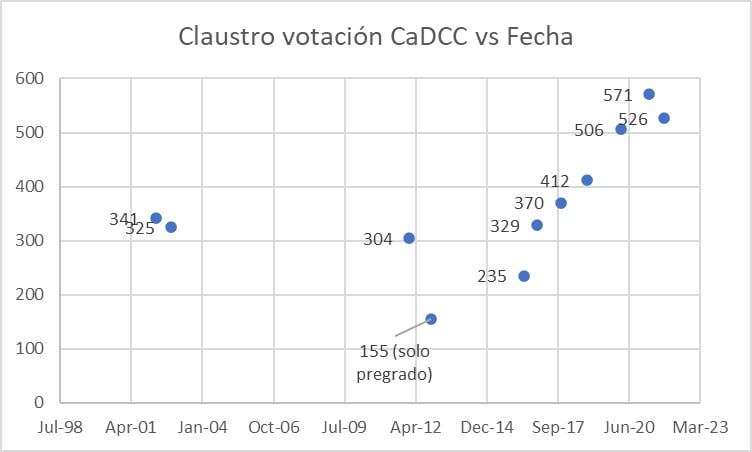
\includegraphics[scale=0.6]{media/imagenes/claustro_votacion_cadcc.jpg}
        \caption[Claustro votaciones \acrshort{cadcc}]{Claustro de las votaciones cadcc desde el 2002 hasta la fecha.}
        \label{fig:aumento_alumnos}
    \end{figure}

\section{Contexto}\label{sec:intro-con}
    \par Uno de los focos de estos desafíos son los procesos de titulación \cite{ARANCIBIA2021}. Asociados a ellos, encontramos informes con reglas de formato, un tipo específico de contenido, procedimientos, pagos, regularizaciones, que junto a otros elementos causan incertidumbre a los alumnos. En relación con ellos, hay varias fuentes de información que atañen a diversos aspectos de estos trabajos, como la wiki de titulación, las páginas del centro de alumnos, publicaciones oficiales en U-Cursos, etc. A pesar de tener estos recursos disponibles, muchas veces, la mayoría de los estudiantes suele preguntar directamente a sus profesores y, funcionarios como la secretaria del departamento suelen recibir la mayor cantidad de dudas no resueltas \cite{ARANCIBIA2021}.
    
    \par Una de las soluciones a considerar, podría ser ampliar personal, lo cual debe ser debidamente justificado, y consensuado \cite{Chile2014}. Por otra parte, tampoco es lo que buscan los estudiantes, pues a la mayoría le gustaría un acceso directo a la información sin pasar por intermediarios \cite{ARANCIBIA2021}. Y es justamente en este ambiente, que el proyecto Mesa de Ayuda Virtual, se posiciona como una buena alternativa para asistir a los estudiantes.
    
    \par El proyecto Mesa de Ayuda Virtual, es un proyecto de soporte o asistencia digital, iniciado por Pablo Arancibia Barahona (egresado del DCC), que busca responder a la necesidad de mejorar el proceso de titulación de alumnos(as). Actualmente está dividido en dos áreas: La primera es un \textit{bot} de \textit{Telegram}, con funcionalidades como preguntas frecuentes agrupadas por proceso, capacidad de feedback por parte del usuario y contactar a un asistente. La segunda, es una página web, que cuenta con un \textit{front-end} para alumnos y otro para administradores, en ellos se puede categorizar preguntas, acceder y modificar los procesos vigentes con sus preguntas, dispone de chat directo con los estudiantes (que usen el bot), entre otros.
    
    \par Este proyecto responde a las necesidades del estudiantado, pues fue diseñado a partir de la información levantada en el departamento y la consideración de las necesidades allí expuestas. Fue validado por la docencia y el centro de estudiantes y, ha finalizado su primera etapa de desarrollo. Actualmente, soporta más procesos como prácticas profesionales.

    \begin{figure}[h]
        \centering
        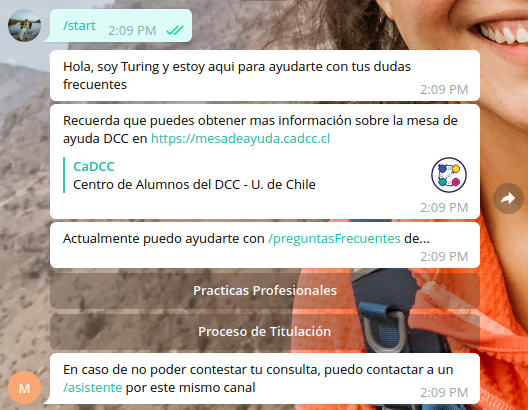
\includegraphics[scale=0.3]{media/imagenes/sc/inicio_bot.png}
        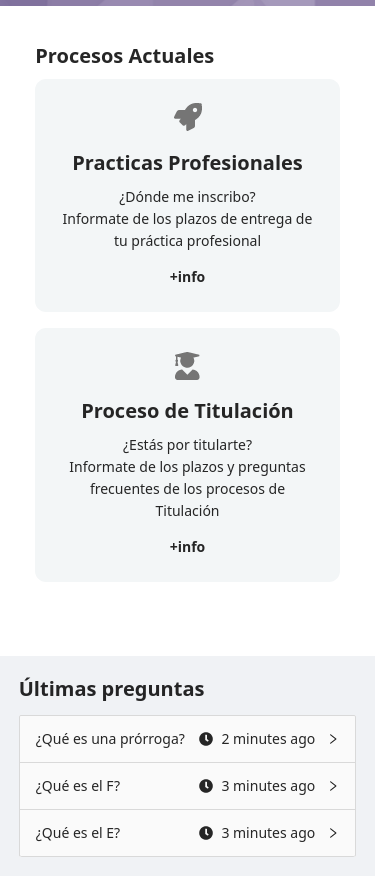
\includegraphics[scale=0.3]{media/imagenes/sc/mesa-de-ayuda-front-mobile-recorte.png}
        \caption[Vista inicio del \textit{bot} y página web]{Imágenes de vista de inicio del \textit{bot} y de la página web de la mesa de ayuda.}
        \label{fig:home-img-bot}
    \end{figure}

\section{Problema}\label{sec:intro-pro}
    \par Como se habló anteriormente, la solución consta de dos partes vitales la web y el \textit{bot}. Dentro de las conclusiones más relevantes del trabajo de Arancibia, destaca el hecho de que la mayoría de los encuestados, dijo que optaría por usar el servicio del \textit{bot} de \textit{Telegram}. Sin embargo, este proyecto no está implementado y presenta algunas falencias en su desarrollo que impiden hacerlo extensible, principalmente en el código del bot. En ese sentido, el que una parte vital del proyecto no pueda tener soporte es algo crítico. 
    \par Además la ausencia de personalización, en un sistema de información, podría hacer que los usuarios lo dejen de usar, ya que este es un factor clave en un sistema como este \cite{Paz2021}.
    \par El presente trabajo busca aportar en la continuidad del proyecto, enfocándose en resolver los problemas descritos en los objetivos.

\section{Objetivos}\label{sec:intro-obj}
  \subsection*{Objetivo General}\label{sec:obj-g}
       El objetivo general es extender el sistema actual, agregando funcionalidades que permitan crear un sistema extensible, personalizado y confiable. El cual será actualizado principalmente por el \acrshort{cadcc}, con miras de integrar otros actores posteriormente, favoreciendo la continuidad de este servicio.
        
    \subsection*{Objetivos Específicos}\label{sec:obj-e}
        \begin{enumerate}
            \item Analizar la solución existente, con el fin de identificar qué modificaciones son relevantes, tanto para que el modelo de datos soporte las nuevas funcionalidades, como para saber la manera en que se debe reestructurar el código.
            
            \item Rediseñar los modelos y funcionalidades, para que el sistema acepte las modificaciones necesarias.
            
            \item Diseñar nuevos componentes de confiabilidad que permitan añadir información a las respuestas y mejorar el modelo de feedback del usuario, para que se pueda obtener más información como su vigencia.
            
            \item Diseñar un modelo de subscripción personalizada: que contempla una búsqueda personalizada de procesos, un elemento suscriptor, variables relevantes de notificar y un modelo de notificaciones y data del alumno, entre otras \textit{features} relevantes para los alumnos.
            
            \item Implementar y probar las reestructuraciones, asegurando la integridad del modelo de datos, del código y permitiendo su extensibilidad a través de la modularidad lógica.
            
            \item Implementar y probar las nuevas funcionalidades buscando que sean aquellas relevantes para los alumnos.
        \end{enumerate}
         
    \subsection*{Evaluación}\label{sec:eval}
    Para validar que el objetivo se cumplió, hay dos áreas que tomar en cuenta: La integridad del sistema y la validez de las nuevas funcionalidades.
    \par En relación con la primera, se espera que las modificaciones hechas le permitan al sistema seguir cumpliendo con sus objetivos. Para lo cual se creará y usará una serie de tests que permitan asegurar sus funcionalidades críticas y la integridad del sistema. Por ejemplo, en el \textit{back-end} probando los \textit{end-points}, que los modelos permitan operaciones \textit{CRUD}, entre otros.
    
    \par En relación con la validez de las nuevas funcionalidades, se propone hacer tests de usabilidad, tanto entrevistas individuales como \acrlong{f}.
    
    \par Adicionalmente, solo si es posible, se propone beta testing, porque permitiría integrar ambas áreas y acercar el producto al usuario. Pero esto depende de la disponibilidad del \acrshort{cadcc}, así como de que el sistema ya esté desplegado por ellos.

\section{Solución Propuesta}\label{sec:intro-sol}
    \par Para poder llevar a cabo los objetivos anteriormente descritos, se propone agruparlos en 3 fases: Análisis, Diseño e Implementación. Pensadas en la lógica que abarca cada uno de estos objetivos.
    
    % Modificaciones
    \par El Análisis tiene el propósito de asegurar la mantenibilidad y rescatar las funcionalidades críticas. Para lo cual, se estudiará en detalle la solución actual. Con esto se busca identificar todos aquellos aspectos relevantes, así como aquellos que necesiten una modificación, ya sea una reestructuración o reimplementación. Entre ellos: las modificaciones en el modelo de datos, las refactorizaciones en el código para modularizar la solución actual y darle una estructura lógica, que permitan entender el sistema y hacerlo extensible.
    
    \par A partir de este proceso, se diseñarán y usarán tests que sirvan para validar como el sistema actual responde a los objetivos originales y los planteados en esta propuesta. Luego con el conjunto de test diseñados, cuando existan modificaciones, se probará que no afectaron la funcionalidad original ya implementada.
    
    % Features de confiabilidad
    \par Durante el Diseño,  se buscará agregar elementos de confiabilidad y generar un modelo de subscripción.
    
    \par Para mejorar la confiabilidad se agregará a las respuestas, la fuente de la información y su última actualización. Y junto con esto, la capacidad del usuario de retroalimentar al sistema, permitiendo ayudar a establecer métricas de vigencia reales, basadas en las calificaciones de los usuarios, así como proporcionar ayuda a los administradores del sistema, al poner atención a aquellos procesos que requieren realmente una actualización, lo que permite enfocar los esfuerzos.
    
    \par Se creará un modelo de subscripción, este permitirá buscar y seleccionar un proceso de forma individual, por ejemplo: \guillemotleft El proceso de titulación otoño 2022\guillemotright.  A partir de esta búsqueda, se debe permitir suscribirse no solo al proceso global, sino que de forma más específica a información que sea relevante para el alumno, por ejemplo: fechas de entrega, requisitos, consecuencias, entre otros\footnote{A estos elementos se les denominó \guillemotleft elemento subscriptor\guillemotright en los objetivos.}.
    
    \par Así mismo, hay que generar un modelo de notificaciones, que se ajuste a estas necesidades, y que sea lo suficientemente simple como para poder extenderlo sin problemas.
   
    \par Al final de esta fase, se debe validar estos modelo con usuarios, y entidades relevantes para hacer un ajuste, antes de comenzar con la etapa de implementación. Estas validaciones deben contemplar todos los aspectos ya mencionados como nuevas funcionalidades, centrándose en la relevancia de cada una para del estudiante. Al mismo tiempo, el agregar nuevas funcionalidades y personalización que dependa de datos del usuario, puede levantar problemas de privacidad que deben ser revisados junto a los encuestados.
    % Implementación

    \par La última fase es la implementación de las funcionalidades ya validadas. Este proceso busca integrar estas funcionalidades, tanto al \textit{back-end} como al \textit{front-end}. Por lo tanto, nuevamente se requerirá de un alto grado de cuidado para no romper las funcionalidades ya implementadas.
    % Validación
    \par Estas \textit{features} deben ser testeadas. Además se incluirá un proceso de validación con los usuarios que incluya demos. Opcionalmente, pero no depende del memorista, se plantea la posibilidad de incluir estas funcionalidades en un sistema de producción. Pero esto depende del \acrshort{cadcc} y de la disponibilidad de sus miembros.
    % Documentación y extras.
    \subsection{Documentación}
    \par Aunque la documentación no representa un desafío técnico elevado, se quiere destacar su rol, en la extensibilidad de un sistema, por lo que, se requiere tiempo, especial en cada iteración, para realizar una buena documentación del sistema.
    % Dentro de otros aspectos no fundamentales este sistema incluirá una forma de auditar el tiempo de respuesta, las fuentes de información confiable, identificación y preferencias de los usuarios, así cómo métricas de uso para su mejora continua.
    
    \subsection{Tecnologías}
        Si bien la decisión de qué tecnologías usar, puede verse modificada en un futuro, según los resultados del trabajo, en primera instancia se pretende continuar con el \textit{setup} original del proyecto.\\
        Dentro de los lenguajes a utilizar se destacan: Python y JavaScript. Estos están fuertemente ligados a las herramientas que se usan en los distintos aspectos del proyecto.
        \begin{itemize}
            \item \textbf{Servidor}: El servidor funciona principalmente en \textit{\gls{Django}}, a través de la librería \textit{Django channels} se sincronizan los chats del administrador con el bot. También se pretende integrar \textit{\gls{Celery}} para el menejo de procesos asíncronos.
            \item \textbf{Motor de Base de datos:} La base de datos, inicialmente pensada para preguntas repetitivas y frecuentes, usa \textit{MongoDB}, que como herramienta \textit{NoSQL}, está especializada en este tipo de \textit{requests}. También, puede que sea necesario agregar otro tipo de motores en el transcurso del proyecto, ya que hay varias áreas sobre todo auditoría, en las que el modelo, no se ajusta completamente al enfoque \textit{NoSQL}.
            \item \textbf{Cache sesión usuario}: Se usa \textit{Redis}, para administrar las conversaciones a través de \textit{Django Channels}.
            \item \textbf{Pagina Web}: La página web, esta principalmente diseñada en \textit{React}, más algunas librerías para facilitar el desarrollo de componentes visuales. Se destaca, que idealmente esta no se encuentra en el scope del proyecto.
            \item \textbf{Telegram API}: Telegram provee de una API la opensource la que se conecta a través de websockets con el servidor.
        \end{itemize}

\section{Metodologías}\label{sec:intro-met}
    \par Para implementar lo propuesto se dividió el proyecto en 4 partes: Primero se realizó un levantamiento y análisis de datos, a partir de aquello un diseño basado en las preferencias de usuario, luego se analizó y reestructuró el código. Finalmente se realizó la implementación de las nuevas funcionalidades.

    \par Para realizar el levantamiento de información, se convocó a dos \acrlong{f}, cuyos resultados se pueden ver en la sección \ref{sec:focus}. Luego se agruparon las respuestas de los estudiantes a las diferentes materias, en áreas de interés y tópicos críticos del sistema. Después, se elaboró un análisis sobre las opiniones conjuntas de los estudiantes. Con esto se hizo una clasificación cualitativa de los estudiantes, y se resumieron sus preferencias, objetivos y funcionalidades deseadas al final de la sección correspondiente.

    \par A partir de los datos obtenidos y su análisis posterior, se generalizaron los objetivos de los estudiantes en 4 diagramas. Estos contienen sus percepciones en torno a la manera de  cumplirse esos objetivos y lo que se complementa con las funcionalidades disponibles del bot, para esquematizar la manera en que se debe realizar el desarrollo de software. Las conclusiones obtenidas en el desarrollo de este análisis permitieron hacer una implementación centrada en los objetivos del usuario.

    \par Luego se analizó en profundidad el código existente, se hicieron varias pruebas funcionales y se modificó parcialmente el código para albergar nuevas funcionalidades. A partir de este trabajo preliminar, se desarrolló una reimplementación profunda separando en capas lógicas el procesamiento de la información, lo que se dividió de las acciones que el sistema realiza a partir de las peticiones del usuario (ver sección \ref{sec:imple}).

    \par Finalmente se realizó la implementación de las nuevas funcionalidades de suscripción, se añadió documentación durante el trabajo y se realizaron una serie de correcciones de compatibilidad, para asegurar el resultado.


\chapter{Marco Teórico}\label{mt}
\section{Estado del Arte}
    \par Para el desarrollo de este trabajo se hizo una investigación sobre los sistemas que solucionan problemas similares y a que objetivos responden. Al mismo tiempo como abordar el hecho de que el usuario es parte fundamental del flujo del sistema tanto en su funcionamiento como imponiendo restricciones dinámicas sobre el mismo, las que responderían a preferencias o valores de cada usuario\footnote{Esto se extrae del trabajo con alumnos, ver \ref{sec:focus}}. Por este motivo los temas abordados e investigados a continuación son \textit{\acrfull{UCD}}, \textit{human in the loop}, \textit{information systems} y \textit{chatbots}.
    
    \subsection{Requisitos diseño centrado en el usuario}
    \par Este es un sistema que indudablemente se basa en el usuario y sus preferencias, es por esta razón que para que el desarrollo sea exitoso no basta con que se desarrolle de la manera correcta y asumiendo buenas prácticas, sino que debe hacerse en torno al usuario y rescatando no solo su input \cite{Karat1997}, sino sus objetivos y valores. Dentro de las maneras de enfocar un desarrollo centrado en el usuario encontramos 3 alternativas la especialista, generalista y mixto \cite{Fox2008}.
    \par La manera especialista hace referencia a que hay 3 actores encargados del proceso, los usuarios, los encargados de \acrshort{UCD} y el resto del equipo de desarrollo. Por otro lado, la generalista asume dos roles: el de usuario y el de desarrollador encargado de esta área.
    \par En esta línea de \textit{\acrlong{UCD}}, el diseño propiamente tal, se entiende como un proceso, en el que debe estar involucrado el usuario final, de forma constante.
    De modo que la personalización llega a ser \guillemotleft una pieza fundamental del diseño exitoso es aterrizar el desarrollo de \textit{features} y herramientas sobre el valor del usuario final\guillemotright \cite{Kramer2000}.
    \par De aquí se obtiene que el sistema debería ser personalizable, y rescatar lo que sea valorado por los usuarios. Dada la naturaleza del proyecto, se decide adoptar un enfoque generalista.
    
    \subsection{El usuario como input del sistema}
    \par Al ser un sistema que depende del usuario para determinar el curso de acción, el humano en este sistema no solo está en ciertos momentos críticos del flujo, sino que es el centro del flujo de información, modelos como este han sido validados con buenos resultados \cite{Smith2018} recientemente.
    \par Los sistemas de información asociados a chatbots, generalmente buscan la integración de información, este proceso es decir mostrarle al usuario una gran variedad de información de diferentes fuentes a través de una vista unificada viene asociado a varias dificultades técnicas y teóricas \cite{Li2017}.
    \par En este sentido, se propone que los sistemas de información que dependen de un humano son altamente complejos, porque los humanos, en este caso usuarios no solo son observadores, sino que tienen la capacidad de incidir en el ambiente no solo reaccionar al ambiente \cite{McBride2021}, sería iluso desarrollar un sistema para las personas sin considerar los objetivos de ellas de forma explícita en el diseño del sistema.
    \par Estos descubrimientos e investigaciones ponen varias restricciones en cuanto al desarrollo de un sistema que depende los usuarios para funcionar y que al mismo tiempo está centrado en el usuario. Pero las podemos condensar en al menos 2: El diseño del sistema debe considerar de forma explícita los objetivos del usuario en cada interacción y debe integrar la información.

    \subsection{Otras aplicaciones de los chatbots en el ámbito académico}
    \par Los chatbots se utilizan desde hace varios años para variados y diversos fines, en múltiples áreas. En particular ahora los abordaremos desde la esfera académica, centrándonos específicamente en instituciones de educación superior.
    En estas se utilizan principalmente como un medio de apoyo al proceso de aprendizaje, como soporte para procesos universitarios, como ayuda para la gestión académica y cómo un sistema de consulta que responde a dudas de diversos entes de estas instituciones.
    \par Como apoyo al proceso de aprendizaje los chatbots se han usado tanto dentro como fuera de la sala de clases.
    \par En la \textit{University of Salerno}, se creó un sistema para responder de manera efectiva las preguntas de los estudiantes, el contexto de \textit{e-learning}. A grandes rasgos es un sistema que usa procesamiento de lenguaje natural como técnicas de ontología, para ligar las preguntas de los estudiantes al contenido disponible y de esta forma poder responder eso que los alumnos están buscando \cite{Clarizia2018}.
    \par El Dr. Sherif Abdelhamid del \textit{Virginia Polytechnic Institute and State University} también propuso un sistema de características similares \cite{Abdelhamid2020}, con las distinciones de que uso el sistema de reconocimiento de voz para traducir las dudas verbales de los estudiantes a texto y así procesarlas y que su objetivo estaba ligados a los elementos que acompañaban el estudio más que al aprendizaje académico en sí. Algunos ejemplos como cuál es la bibliografía pertinente al curso, que recursos tiene disponibles, que debería aprender, etc.
    \par En este aspecto, investigadores del \textit{Department of Mathematics and Computer Science, University of Kabianga, Kericho, Kenya} con miembros del \textit{Department of Curriculum Instruction Educational Media, School of Education, Moi University, Kenya} analizaron la respuesta de los mismos profesores a la introducción de estas herramientas en la rutina de enseñanza \cite{K2018}.
    
    \par Como soporte para procesos universitarios los chatbots se han usado para entregar el horario de clases o las clases siguientes así cómo ayudar a los alumnos a elegir ramos.
    
    \par Desarrolladores de la \textit{Bogdan Khmelnytsky Melitopol State Pedagogical University} en Ucrania, desarrollaron un servicio de 3 capas para poder implementar un servicio de ayuda al entregar el horario de clases a través de un chatbot, esto se hacía no solo con la finalidad de ayudar a alumnos que hayan olvidado o no un horario o su sala, sino también porque los horarios pueden sufrir cambios o modificaciones, además de que si bien hay alternativas simples como fotos estas se pierden en un gran volumen de elementos similares sin relación, lo que las hace difícil de volver a obtener, según la investigación \cite{Priadko2019}.
    
    \par En \textit{The Open University of Hong Kong Hong Kong} desarrolladores implementaron un sistema para facilitar a los alumnos la decisión sobre qué cursos tomar a través de un chatbot \cite{ChunHo2018}.
    
    \par En el área de los desarrollos de ayuda para la gestión académica, se encontraron desarrollos ligados a: Hacer disponibles servicios en horarios no hábiles, Mantener, monitorear y mostrar la información del alumno y Acercar la implementación de chatbots a usuarios de más alto nivel y con menos conocimiento técnico.
    
    \par Los trabajos de Vaishnavi Ajay Inamdar1 y Shivanand R.D en el \textit{BIET College} de la India, van enfocados en poder proveer servicios de gestión académica en cualquier momento, de este modo bajar la carga de los funcionarios y proveer de una \textit{\gls{effectiveGUI}} \cite{Journal2019}.
    
    \par Del \textit{Engineering Rajalakshmi Institute of Technology} una profesora y sus alumnos, desarrollaron un sistema para administrar la información escolar de los alumnos y está ligado la base de datos de administración. Este sistema tenía el foco en el personal administrativo de la institución y dependía de la información entregada por el alumno.
    
    \par Con el foco en los apoderados o tutores de un alumno, en la \textit{Universitas Komputer Indonesia} A Heryandi, desarrolló un sistema de chatbots para poder desplegar las notas y el rendimiento de los alumnos a los padres usualmente menos versados en tecnología y más familiarizados con plataformas de mensajería. Por esto mismo se desarrolló un sistema con \textit{Easy access}, es decir, con un login o un proceso de autenticación sencillo y con información conocida por los tutores \cite{Heryandi2020}.
    
    \par En Indonesia en la \textit{Universitas Sebelas Maret} investigadores desarrollaron un sistema con un bot de Telegram para incluir a funcionarios no expertos en el diseño de funcionalidades para la universidad. Este proveía funcionalidades como agregar botones, comandos, acciones, mensajes directos, transmitir mensajes, configuraciones y análisis \cite{Hasyim_2021}.
    
    \par Como un sistema de consulta se han desarrollado sistemas de preguntas frecuentes, algunos ejemplos son el sistema de Mesa de ayuda del DCC \cite{ARANCIBIA2021} y un trabajo de la \textit{Manipal University} en la India \cite{Ranoliya2017}.
    \par Aunque ambos son similares, responden a necesidades completamente distintas, el sistema del DCC es un proyecto centrado en el usuario, mientras que el trabajo de la India tiene un foco en la performance y el uso de IA.
    
    \subsection{Análisis de las aplicaciones actuales}
    \par Como se puede observar los bots cumplen variadas funciones dentro de la vida universitaria a través del mundo, apoyando a toda la comunidad escolar, tanto tutores, como funcionarios y alumnos, haciendo más accesibles, disponibles y eficientes diversos servicios, incluso apoyando procesos de aprendizaje virtual y presencial.
    \par A pesar de la gran diversidad de funcionalidades que están presentes en estos sistemas, se logra rescatar que en la mayoría de los casos se diseña basándose en un modelo de inputs, procesamiento y respuestas. En la mayoría de los casos a pesar de ser desarrollos que buscan acercar o facilitar la vida de sus usuarios, suelen tomar un enfoque técnico y centrarse en aspectos como tener una \textit{\acrshort{effectiveGUI}}, son desarrollos que en general carecen de un modelo que integre al usuario directamente, y se enfocan en solucionar los problemas de manera analítica o teórica. Esto podría ser una enorme dificultad para el proyecto e iría en contra de los descubrimientos en el área de \textit{\acrlong{UCD}}.
    \par Por estas razones se opta por tomar los buenos resultados funcionales de los chatbots, pero agregarles de alguna forma las preferencias de los usuarios de forma explícita en el diseño de los nuevos modelos de interacción.

\section{Notacion i*}
    \par La notación \gls{i*}, se usará como se mencionó anteriormente para explicar no solo la interacción del usuario con el sistema, sino también, qué persiguen los mismos al realizar dicha interacción.
    \par Las bases del lenguaje se pueden encontrar en la guía del lenguaje \cite{Dalpiaz2016} y las imágenes en la wiki del lenguaje \cite{No-mention2011}.
    \par Esto se hace a través de la sintaxis de este lenguaje que detallaremos brevemente a continuación:
    \begin{itemize}
        \item Objetivos: los objetivos o \textit{Goals} por su nombre en inglés, son en palabras simples un estado que desea alcanzar, por el usuario en relación con algo. Por ejemplo: \guillemotleft Tener los pasajes de avión comprados\guillemotright.
        
        \begin{figure}[H]
            \centering
            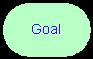
\includegraphics{media/imagenes/i_star/sintaxis/goal.jpg}
            \caption{Objetivo \gls{i*}}
            % \label{fig:my_label}
        \end{figure}

        \item Tareas: las tareas (\textit{Task}) son acciones que el usuario puede realizar para lograr su objetivo. Ejemplo: \guillemotleft Buscar pasajes de avión\guillemotright, \guillemotleft Comprar pasajes en la aerolínea\guillemotright.
        
        \begin{figure}[H]
            \centering
            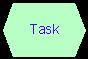
\includegraphics{media/imagenes/i_star/sintaxis/task.jpg}
            \caption{Tarea \gls{i*}}
            % \label{fig:my_label}
        \end{figure}
        \item Cualidades: o \textit{Qualities} son maneras o elementos de valor que se quiere preservar u obviar al completar un objetivo. Ejemplo: \guillemotleft Rápido\guillemotright, en esta serie de ejemplo la frase completa se entendería como \guillemotleft Tener los pasajes de avión comprados rápido\guillemotright o de manera \guillemotleft rápida\guillemotright.
                \begin{figure}[h]
            \centering
            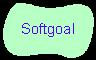
\includegraphics{media/imagenes/i_star/sintaxis/softgoal.jpg}
            \caption{Cualidad \gls{i*}, antes \textit{softgoal} en i* 1.0}
            % \label{fig:my_label}
        \end{figure}
        \item Recursos: Los recursos son elementos ligados a las tareas, como una \guillemotleft tarjeta de crédito\guillemotright en esa línea se podría \guillemotleft comprar los pases en la aerolínea con una tarjeta de crédito\guillemotright.
                \begin{figure}[h]
            \centering
            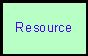
\includegraphics{media/imagenes/i_star/sintaxis/resource.jpg}
            \caption{Recurso \gls{i*}}
            % \label{fig:my_label}
        \end{figure}
        
        \item Actores: Los actores son elementos principales del diagrama, realiza acciones, dispone los recursos y tiene objetivos. Pueden ser de tres tipos: un tipo general cuando no se desea especificar, un agente que representa una instancia particular de un actor: como \guillemotleft Juan\guillemotright o el\guillemotleft Bot\guillemotright y un rol, que viene a ser una categoría o clase como \guillemotleft Estudiante\guillemotright.  Las \textit{boundaries} o límites relativos a un actor determinan que elementos le \guillemotleft pertenecen\guillemotright.
        
        \begin{figure}[h!]
            \centering
            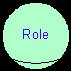
\includegraphics[scale=0.4]{media/imagenes/i_star/sintaxis/role.jpg}
            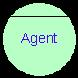
\includegraphics[scale=0.4]{media/imagenes/i_star/sintaxis/agent.jpg}
            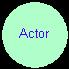
\includegraphics[scale=0.4]{media/imagenes/i_star/sintaxis/actor.jpg}
            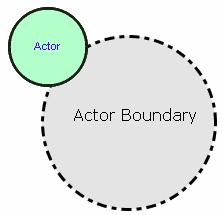
\includegraphics[scale=0.4]{media/imagenes/i_star/sintaxis/actorboundary.jpg}
            \caption{Actores \gls{i*}}
            % \label{fig:my_label}
        \end{figure}
        
        \item Enlaces: o \textit{Links} son lo que representa las relaciones entre los diferentes elementos del sistema, pueden representar dependencias, contribuciones, especificaciones o incluso notar una contribución. En el caso de este trabajo se usan principalmente 3 tipos de enlaces:
        \begin{itemize}

            \item Dependencias: Se indican con una letra D y expresan que el elemento a la izquierda de la dependencia, depende del elemento a la derecha, de manera un poco simplista.
            \begin{figure}[h!]
                \centering
                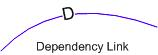
\includegraphics[scale=0.6]{media/imagenes/i_star/sintaxis/dependencylink.jpg}
                \caption{Dependencia \gls{i*}}
                % \label{fig:my_label}
            \end{figure}

            \item Contribuciones: Indican que cierto elemento contribuye a una Cualidad, puede ser de 4 formas, satisfaciendo completamente lo que se nota con \textit{make} sobre el enlace, Imposibilitando su realización lo que se denota con \textit{break}, o ayudando un poco o debilitando un poco lo que se denota con \textit{help} y \textit{hurt} respectivamente.
            \begin{figure}[h!]
                \centering
                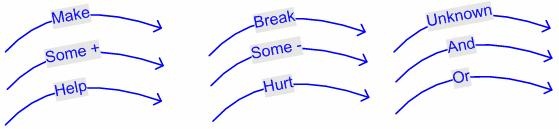
\includegraphics[scale=0.6]{media/imagenes/i_star/sintaxis/contribuitonlinks.jpg}
                \caption{Contribuciones \gls{i*}}
                % \label{fig:my_label}
            \end{figure}
            
            \item Refinamiento: Expresan que un objetivo o tarea tiene otros elementos que lo definen. Pueden ser O (\textit{OR}) o Y (\textit{AND}), lo que determinan es que para que el objetivo se satisfaga se debe satisfacer a su vez todos los elementos que lo refinan (\textit{AND}) o alguno de ellos (\textit{OR}).
            \begin{figure}[h!]
                \centering
                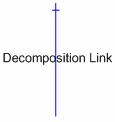
\includegraphics[scale=0.6]{media/imagenes/i_star/sintaxis/decomposition.jpg}
                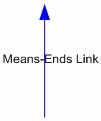
\includegraphics[scale=0.6]{media/imagenes/i_star/sintaxis/meansendslink.jpg}
                \caption{Refinamiento \gls{i*}}
                % \label{fig:my_label}
            \end{figure}
        \end{itemize}
    \end{itemize}

\chapter{Trabajo Previo}
 En este capítulo, se resumen los alcances del proyecto mesa de ayuda iniciado por Pablo Arancibia y acogido por el \acrshort{cadcc}. Se divide en los detalles relevantes de la solución existente y los alcances de esta plataforma.
\section{Solución existente}
    El proyecto iniciado el 2020, cuanta esencialmente con un diseño basado en una arquitectura de 4 partes: Database, back-end, aplicación web y el bot. El Modelo de datos se basa principalmente en la información que el sistema consume, credenciales de usuarios y feedback de los usuarios de bot. Este sistema es una gran mejora a las vías actuales de información de los alumnos, principalmente porque está diseñado para responder las dudas de los estudiantes de manera satisfactoria, mejora la comunicación entre alumnos y funcionarios, además de estar validado por la comunidad del \acrshort{dcc} \cite{ARANCIBIA2021}.

    \subsection{Arquitectura Previa}
        \begin{figure}[h]
            \centering
            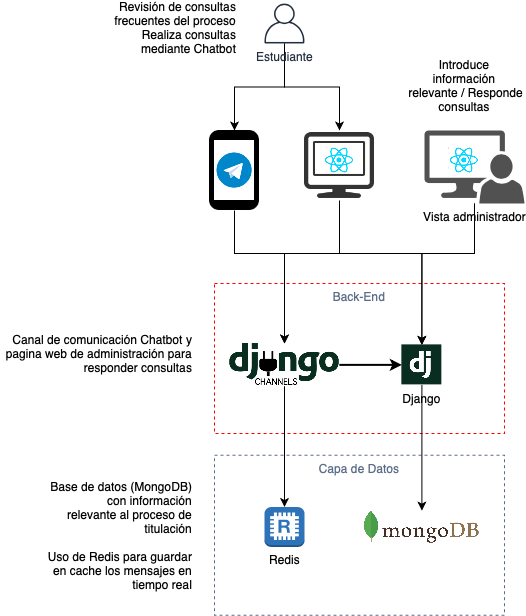
\includegraphics[scale=0.5]{media/imagenes/trabajo_previo/arquitectura_del_sistema.png}
            \caption[Arquitectura sistema anterior]{Esquema de arquitectura del trabajo realizado por Pablo Arancibia. Obtenido desde \cite{ARANCIBIA2021}}
            \label{fig:arc-previa}
        \end{figure}

        \par Cómo se puede observar en la figura \ref{fig:arc-previa}, la capa de datos cuenta con dos bases de datos: Redis y Mongodb. Redis se usa para guardar mensajes en caché en tiempo real, enviados por ejemplo desde un estudiante a través del bot a un asistente en la plataforma de administración web. Mientras que Mongo se usa para almacenar la información relevante de los procesos, las cuentas de los usuarios, los mensajes de los usuarios de forma persistente, etc.
        \par El back-end hecho en Django, sirve tanto al bot, la plataforma web de estudiantes y administración. Aquí se utiliza la tecnología de django channels para sincronizar mensajes desde el bot a la vista web. Django principalmente se usa para manejar las consultas a la base de datos por información, cómo el procesamiento y traspaso de mensajes desde el bot.
        \par El front por otra parte se divide entre la plataforma de telegram y el front diseñado en react, para la vista de alumnos y administración. El Bot utiliza la API de \gls{Telegram} para generar vistas e interactuar con el usuario. La plataforma web por otra parte es una aplicación completa que muestra información sobre el proceso además de proveer el módulo de administración, para contestar mensajes, editar la información, entre otras.

    \subsection{Modelo de Datos Previo}
        \begin{figure}[h]
            \centering
            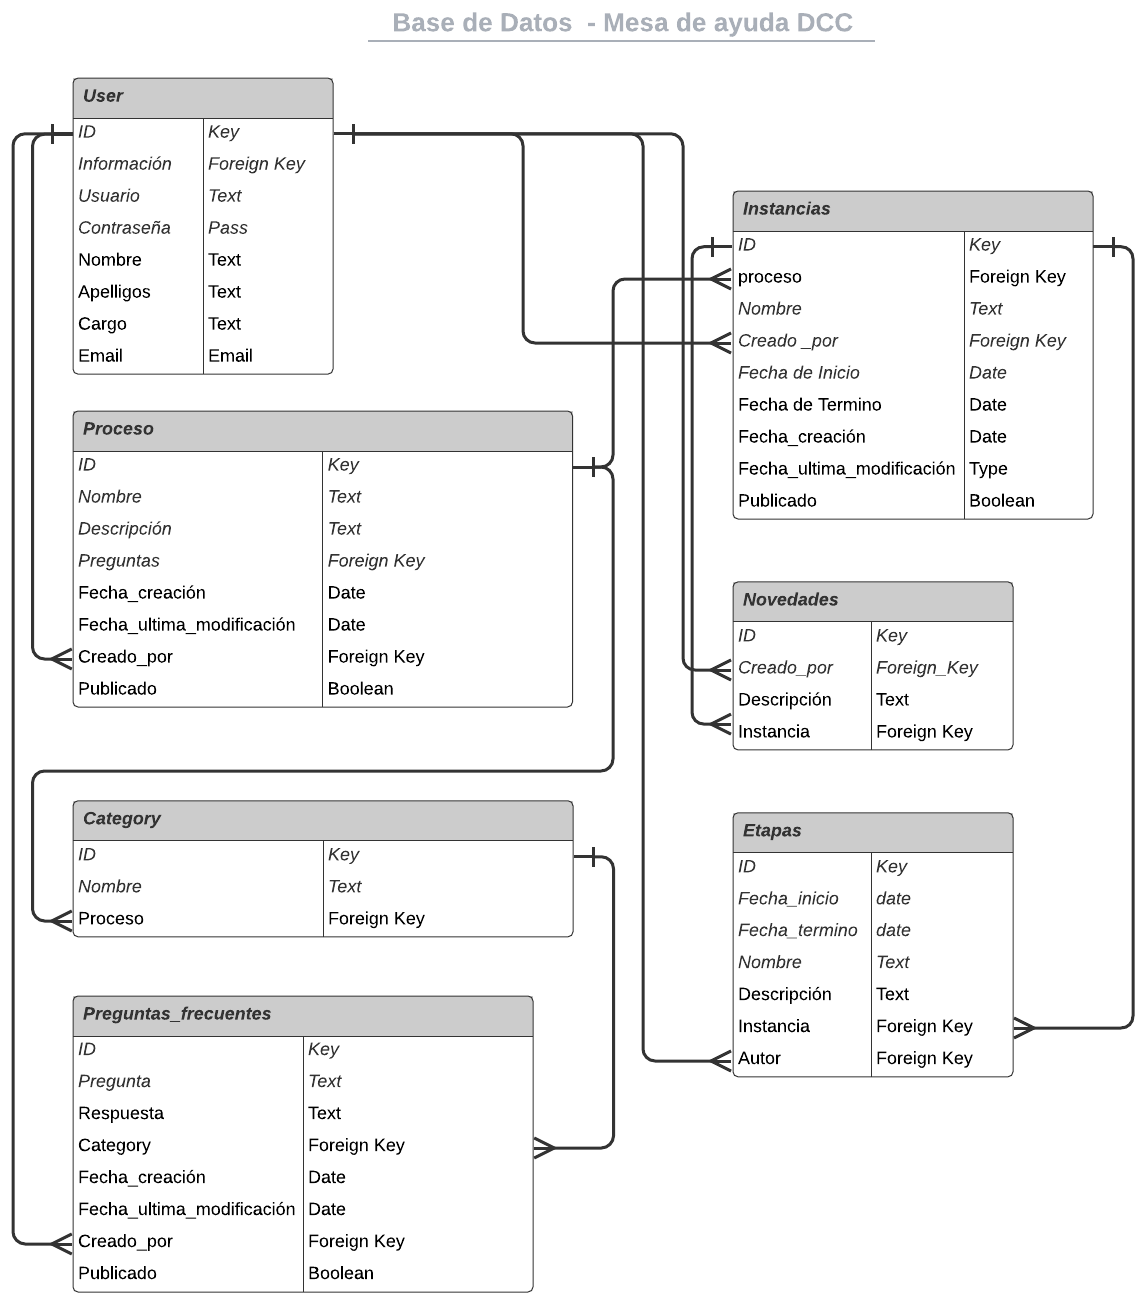
\includegraphics[scale=0.25]{media/imagenes/trabajo_previo/modelo_datos.png}
            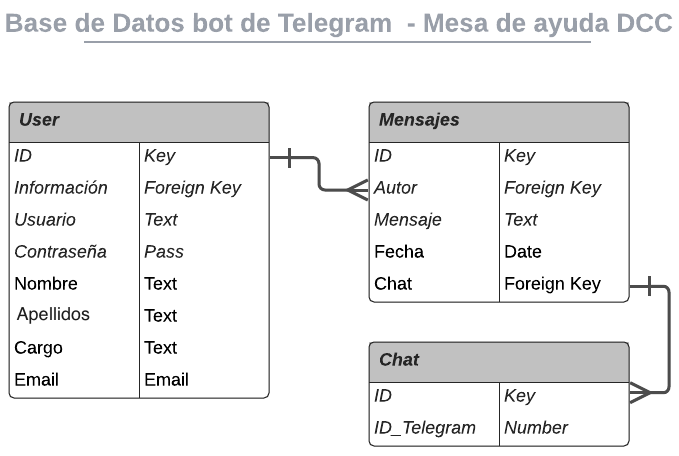
\includegraphics[scale=0.25]{media/imagenes/trabajo_previo/modelo_datos_bot.png}
            \caption[Modelo de datos]{Modelo de datos del trabajo realizado por Pablo Arancibia. Obtenido desde \cite{ARANCIBIA2021}}
            \label{fig:md-previo}
        \end{figure}
        
        \par El modelo de datos se puede estudiar en detalle en \cite{ARANCIBIA2021}, pero a grandes rasgos. Tiene las credenciales de los usuarios de administración \footnote{tabla user} y la información de los procesos.
        \par La información de los procesos académicos, esta distribuida en 2 grandes áreas, aquella que es semi estática\footnote{Se dice semi estática y no completamente estática, porque la información en la base se puede modificar, sin embargo, es transversal a la fecha de consulta o de realización de un proceso.} en el tiempo y la que cambia continuamente. 
        \par La información relacionada con un proceso, cómo por ejemplo \guillemotleft Proceso de Titulación \guillemotright o \guillemotleft prácticas profesionales \guillemotright es el nombre, la descripción, las preguntas frecuentes y las categorías de estas preguntas frecuentes. Por otro lado, una instancia del proceso, cómo por ejemplo  \guillemotleft Proceso de Titulación 2022 \guillemotright, tiene asociadas las novedades y las etapas de dicho proceso, ya que estas van a variar de instancia a instancia.

    \subsection{Módulos lógicos del bot}
        \begin{figure}[h!]
            \centering
            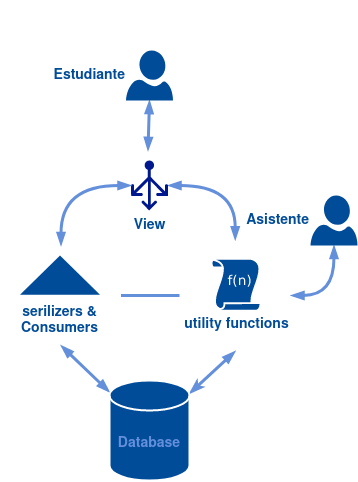
\includegraphics[scale=0.5]{media/imagenes/trabajo_previo/Bot_Modules-old.png}
            \caption[Funcionamiento del Bot]{Diagrama que esquematiza el funcionamiento del bot.}
            \label{fig:bot-work-old}
        \end{figure}
        \par la aplicación del bot, actualmente cuenta con los scripts default de Django más routing utilziado por django channels, además de \textit{consumers} y \textit{serializers} que se usan para seguir un estándar \gls{REST}.
        \par los \textit{scripts consumers} y textit{serializers} engloban la lógica de serializar los datos y procesar las \textit{requests} y la data anexa de json para traducirlas a \gls{Django}. Por otra parte routing es utilizado en caso de que sea necesario establecer un websocket entre la aplicación web y el servidor para mantener una comunicación en tiempo real entre el administrador y el alumno.
        \par en el modulo view, se hace el procesamiento de los \textit{requests}, actualmente engloba la mayoria de las operaciones y funciones del bot como eviar mensajes, procesar input del usuario, extraer data para el chat desde la base de datos y guardar inputs en ella.

    \subsection{Problemas del trabajo previo}
        \subsubsection{Falta de modularización}
            \par El bot, cómo estaba desarrollado, incluía la mayoría de las funciones nucleares en la \textit{view} de \gls{Django} (ver \ref{list:view}). Esto implica que no es claro dónde se podría modificar el código para agregar nuevas funcionalidades. Si se desea mantener el diseño, la única forma de extender el código es añadiendo nuevas funciones o modificando las existentes, sin mejorar el orden lógico. Esto tácitamente implica que para cada cambio grande se debe hacer un \textit{refactoring} del código actual. Además lo hace poco legible, hace que trabajar simultáneamente en el proyecto implique hacer \textit{branch} y \textit{merges} en un sistema de versionamiento por ejemplo, a pesar de que dos personas trabajen en áreas similares. Estas deficiencias hacen que el proyecto no sea escalable, no por arquitectura física o capacidades del sistema, sino porque no porque la única forma de lograr extender el sistema de forma ordenda y manteniendo la integridad del mismo, es modificar la disposición del código existente. 
            
        \subsubsection{Ausencia de delegación de responsabilidades}
            \par Ya que la mayoría de las funcionalidades del bot, se encuentran todas bajo el mismo \textit{script} y además bajo el \textit{scope} de la función principal de la view. La única forma de procesar distintos protocolos de comunicación o formas de procesar mensajes, es través de condicionales sobre el contenido del código, esto implica que la ramificación y extensión de la función principal puede crecer indefinidamente a medida que se deseen agregar nuevas formas de entendimiento, cómo comandos de telegram o procesamiento de lenguaje natural.
            \par También implica que la lógica de acción a realizar depende de la misma capa en el sistema, por lo tanto, al ir añadiendo funcionalidades se crea una sobrecarga sobre esta parte de la API. Asi mismo resulta difícil agregar nuevos comportamientos sin extender el código existente, lo que hace aún menos claro cómo funciona el procesamiento de mensajes.
        \subsubsection{Ausencia de Documentación}
            \par El sistema actual solo cuenta con un \textit{README}, que tiene la información esencial para ejecutar el proyecto. Pero hay nula información sobre cómo funciona el sistema, sobre cómo se pueden extender los módulos actuales, cómo se comunican las diferentes partes del sistema. Esto hace que el proyecto dependa de que las personas que trabajan en él, deban conocerse y comunicarse continuamente. En el caso de perder esta comunicación el proyecto queda virtualmente desechado, porque la configuración es lo suficientemente compleja, como para hacer difícil que alguien la tome y la extienda sin apoyo de un desarrollador del proyecto. 
            \par Por otro lado muchas de las librerías utilizadas en el sistema están bajo cambios constantes, al punto de que durante el trabajo de esta memoria cambiaron su comportamiento, incluso la documentación de lugar. Algunas se volvieron proyectos con una versión de pago, y eso hace que si alguien que no conoce estas librerías toma el proyecto, le tomará un tiempo largo entender los errores que el sistema puede arrojar. Incluso, pueden iniciarse errores inesperados o \textit{dataraces}, lo que harían al sistema inutilizable. 
            \par Cómo uno de los objetivos es que este sistema sea adoptado por los estudiantes del departamento y extendido por ellos, estas faltas de documentación no pueden existir, porque este material es necesario para mantener, extender y mejorar el proyecto.
            \par Finalmente, las tecnologías utilizadas son variadas y diversas, por lo tanto para alguien no familiarizado con ellas, tienen una curva de aprendizaje media alta. Cada una de estas herramientas es extensa tanto en funcionalidades como en documentación, por lo tanto, esto sumado a los cambios constantes, hacen que el proyecto no sea extensible por terceros.

            \begin{listing}
                \begin{minted}{python}
                    class BotView(View):
                        def post(self, request, *args, **kwargs):
                            try: # access field chat_id
                            except Exception as e:
                            try:# access field label
                            self.message_processing(...)
                            return JsonResponse({"ok": "POST request processed"})
        
                        def message_processing(...):
                            messages = []
                            if label is None:
                            if message == '/start': messages = # [list of messages]
                            elif message == '/preguntasFrecuentes':
                            else: # contactar a un asistente
                            elif label == 'Process':  # [list of messages]
                            elif label == 'Category':  # [list of messages]
                            elif label == 'Question':  # [list of messages]
                            elif label == 'Feedback':  # [list of messages]
                            elif label == 'Helper':  # [list of messages]
                            for msg in messages:
                            self.send_message(msg['text'], t_chat["id"], msg['keyboard'])
        
                        # all functions below are static functions
                        def get_process_keyboard():
                        def get_name_process(id):
                        # Similar for category, other functions
                        def send_message_website(message, t_chat):
                        def send_message(message, chat_id, keyboard_button={}):
                    
                \end{minted}
                 \caption[View sistema anterior]{Resumen del código contenido en la \textit{View} de \gls{Django}}
                 \label{list:view}
            \end{listing}
        

\section{Alcances de la solución existente}
    \par Durante la finalización del trabajo anterior, el trabajo con \acrlong{f}, y en conversaciones con el \acrlong{cadcc}. Los estudiantes se han visto favorables a adoptar la plataforma \cite{ARANCIBIA2021}. Han habido varios comentarios acerca de las funcionalidades que debiera incluir, que mejoras se les podría hacer, pero en general se podría decir que la solución tendría una aceptación tal cual esta, solo que aún le faltarían funcionalidades para reemplazar la mayoría de los otros canales de información.
    \par Si bien la solución existente es viable, aún no ha sido puesta en producción de forma definitiva, aunque está disponible en una versión de desarrollo por el \acrshort{cadcc}.
    

\input{chapters/6-Analisis_y_diseño.tex}
\input{chapters/7-Implementación.tex}
\chapter{Validaciones}

\section{Diseño escalable del Bot}
    \par La nueva arquitectura (ver figura \ref{fig:arc-new}),es un sistema de 3 capas: La capa de usuario, el back-end, la capa de tareas y la capa de datos, mediadas por un \textit{broker} de mensajes. En su conjunto ellas crean un sistema capaz de servir información, de recibir y procesar tareas de manera síncrona y asíncrona. 
    \par La nueva forma de procesar información y de segmentar  las acciones del sistema para responder individualmente a cada necesidad del usuario, sumado a la capacidad añadida de separar la forma de comunicación del sistema, permite añadir: Nuevas formas de procesar información como lenguaje Natural, extender las vías de comunicación existentes como botones y comandos. Al mismo tiempo permite extender las capacidades de procesamiento de información añadiendo la oportunidad de planificar tareas en el sistema, lo que serviría para realizar mantenciones de datos, obtener estadísticas, hacer sistemas de aprendizaje automático, entre otros.
    \par Todo el trabajo de \textit{refactoring} apuntaba a hacer el sistema extensible, a ordenarlo de forma lógica, y a permitir diferenciar entre las distintas capas de procesamiento del sistema, permitiendo su continuidad cómo proyecto para el alumnado del dcc.
    \par A sí mismo la modularización creada para manejar la API de \gls{Telegram}, permite ir añadiendo nuevas funcionalidades en torno a las vías de interacción que facilita la plataforma.

\section{Diseño estratégico para proyectos}
    \par Este proyecto busca la adopción por parte de la comunidad del \acrshort{dcc}, por tanto todo su diseño y capacidades iniciales y nuevas, apuntan a crear un sistema que resuelva las reales necesidades de la comunidad. Sin embargo, su mantención y mejora, dependen de alumnos que no necesariamente estarán en contacto con los desarrolladores anteriores del proyecto. Para esto es imprescindible que el proyecto por sí mismo pueda ser entendido, reparado y extendido por personas que pueden o no conocer las tecnologías del sistema. Las que no conocerán las motivaciones iniciales del proyecto, que no necesariamente están al tato del marco teórico que envuelve al sistema, así cómo de las dependencias que este tiene de librerías y trabajos de terceros.
    \par Para que un proyecto pueda continuar vigente, es necesario que su código sea extensible y mantenible. Pero otra de las contribuciones del trabajo actual, es proveer un marco de diseño y evaluación de las funcionalidades en torno a las preferencias del usuario, la mayoría de las interacciones que el sistema puede proveer al usuario se pueden esquematizar con la sintaxis \gls{i*}, y los diagramas actuales generalizan las interacciones posibles. Sin embargo, aunque no fueran adoptados los diagramas, estos proveen de conceptos claves a la hora de evaluar la forma de interactuar de los estudiantes con el sistema. También, cómo estos afectan la manera de diseñar la solución y, la necesidad de mantener formas alternativas de cumplir los objetivos de cada alumno. Y por sobre todo apuntan a mantener de forma explícita en el diseño los objetivos de los usuarios.
    \par Estas contribuciones están en línea con los hallazgos actuales y con la literatura existente. Permiten por tanto, tomar decisiones estratégicas en torno a este proyecto para la comunidad. Esto es de ayuda para quienes continúen el proyecto, y tiene la intención de servir de apoyo para las generaciones futuras.
    \par En el área de la extensibilidad, se hicieron logros importantes en la documentación del código, que permiten a su vez de forma práctica, levantar el proyecto, configurar los módulos, agregar datos de prueba y usar el proyecto, sin necesidad de conocer todas las tecnologías y plataformas utilizadas.
    \par Todo esto en su conjunto permite que nuevas funcionalidades sean implementadas. Manteniendo un ecosistema favorable tanto para el desarrollador como para la comunidad, y desarrollar piezas de software que no solo cumplan con realizar una acción, sino que se amolden a las preferencias de la comunidad, y de cada usuario particular, proveyendo de valor, para la diversidad de estudiantes del dcc.
    \par Todo esto crea un marco conceptual, que permite hacer evaluaciones estratégicas del proyecto, provee una metodología de diseño y promueve que el sistema pueda ser extendido y mejorado de forma efectiva por los estudiantes que continúen el trabajo.

\newpage
\section{Valor agregado para Usuarios}
    A continuación se muestran solo los flujos vía comandos porque los flujos en botones ya existían en el trabajo anterior.
   
    \begin{figure}[h!]
        \centering
        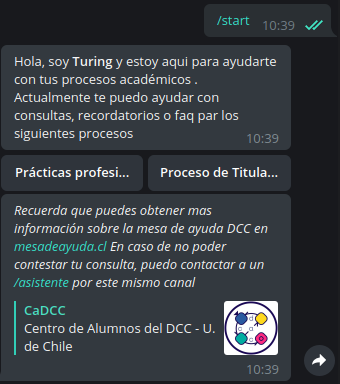
\includegraphics[scale=0.5]{media/imagenes/sc/start.png}
        \caption[Bot start]{Captura de pantalla del Bot Respondiendo el nuevo comando start}
    \end{figure}
    
    \par En el nuevo sistema de procesamiento el bot procesa los comandos en 3 fases. Primero entiende que el usuario ingresa un comando de tipo \mintinline{python}{r'\/command'}. Luego se pasa al handler, el handler determina si es comando aceptado y envía un mensaje como el escrito arriba.

    \begin{figure}[h!]
        \centering
        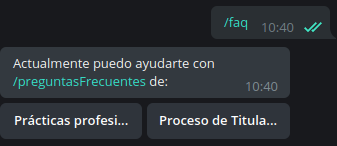
\includegraphics[scale=0.5]{media/imagenes/sc/faq.png}
        \caption[Bot FAQ]{Captura de pantalla del Bot Respondiendo el nuevo comando faq}
        \label{fig:faq}
    \end{figure}

    \par Complementando los flujos de botones se añadieron versiones de comando de las mismas acciones (ver figura \ref{fig:faq}). Además se pueden agregar otras palabras. Pero ambas se procesan de forma completamente diferente (ver sección \ref{imp:refactoring})

    \begin{figure}[h!]
        \centering
        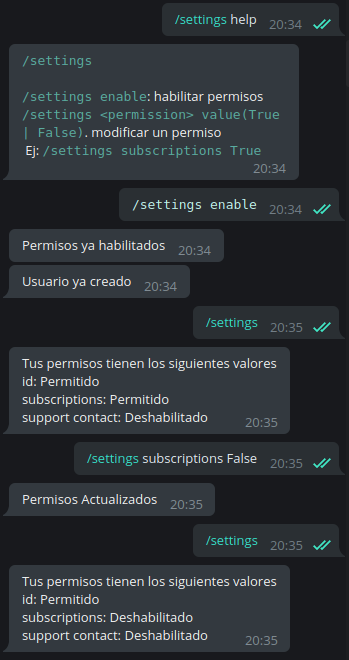
\includegraphics[scale=0.5]{media/imagenes/sc/settings.png}
        \caption[Bot settings]{Captura de pantalla del Bot Respondiendo el nuevo comando settings}
        \label{fig:bot-settings}
    \end{figure}

    \par Además las configuraciones de seguridad y preferencias permiten a los usuarios estar al control de las \textit{features} que requieran, y pueden ser activadas o desactivadas en cualquier momento (ver figura \ref{fig:bot-settings})
    \par Este tipo de configuraciones y funcionalidades, permiten al alumno escoger de que ser informado, segmentar y priorizar la información, y así, se añade valor a este sistema de información.

    \begin{figure}[h!]
        \centering
        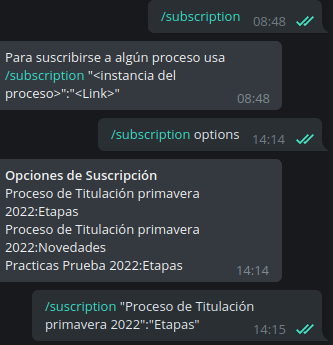
\includegraphics[scale=0.5]{media/imagenes/sc/subscription.png}
        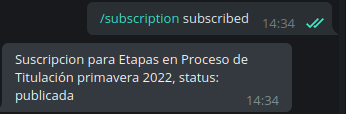
\includegraphics[scale=0.5]{media/imagenes/sc/suscription1.png}
        \caption[Bot subscription]{Captura de pantalla del Bot Respondiendo el nuevo comando subscription}
        \label{fig:bot-sus}
    \end{figure}
    
    \par Se añadió el módulo \textit{BotUsers} a la API, permitiendo que cada alumno pueda escoger la información que es relevante para él. Además ahora puede ser notificado por ejemplo de los plazos de cada proceso. Este módulo contempla que se puedan añadir otras funciones de subscripción como las sugerencias en el futuro. Esto permitiría seguir añadiendo un valor personalizado para cada alumno (ver figura \ref{fig:bot-sus}).

    


\section{Resumen}
    \par De lo expuesto en este capítulo, se puede ver que se satisfacen los requisitos analizado así los cambios necesarios para extender y modificar el sistema, se agregó documentación técnica y lógica al proyecto, se rediseñaron las funcionalidades existentes, y se agregaron nuevas funcionalidades que permiten hacer un sistema extensible, personalizado y confiable.
    \par Además, durante el transcurso del proyecto se sostuvieron conversaciones con las directivas del \acrlong{cadcc}. Y se les presentaron los cambios en el bot, así cómo los problemas de compatibilidad entre otras cosas. El centro de alumnos en conjunto con el memorista anterior, fueron validando los cambios en el código, las nuevas funcionalidades logradas y también apoyaron en la resolución de algunos errores específicos.
    \par Además, cómo se explicita en la memoria, el diseño de las funcionalidades se hizo tomando de forma explícita los objetivos de los alumnos y las cualidades que valoran en estos objetivos.
\chapter{Conclusiones}
\section{Discusión Final}
    \par Con esta memoria se busca seguir mejorando el sistema de mesa de ayuda y, de este modo, mejorar la experiencia de los alumnos durante los procesos académicos, particularmente el proceso de titulación. El objetivo general era \guillemotleft extender el sistema actual, agregando funcionalidades que permitan crear un sistema extensible, personalizado y confiable. El cual será actualizado principalmente
    por el \acrshort{cadcc}, con miras de integrar otros actores posteriormente, favoreciendo la continuidad de este servicio\guillemotright. Para esto se dividió el objetivo principal en 6 objetivos específicos:

    \par En concordancia con el objetivo \href{sec:obj-e}{1}, se analizó la solución existente y se determinaron que las modificaciones necesarias eran: Cambio de procesamiento condicional de la \textit{request}, la separación en capas de procesamiento de mensajes, así cómo la estandarización y modularización de las respuestas del sistema a través de la creación del \textit{Parser}, el \textit{Handler} y los objetos asociados a las acciones.
    \par Se reestructuró el código existente, lo que permitirá la adición de nuevas funcionalidades en el futuro, así cómo extender y mejorar las ya presentes.

    \par Se rediseñaron los modelos actuales, así mismo como las funcionalidades, para que el sistema fuera capaz de recibir las mejoras presentadas en concordancia con el objetivo \href{sec:obj-e}{2}.

    \par  Cumpliendo el objetivo \href{sec:obj-e}{4}, se desarrolló un modelo de suscripción personalizada: El que permite para cada proceso agregar opciones de subscripción a las que el usuario puede suscribirse, así mismo se creó un modelo de notificaciones, y data mínima del alumno para habilitar o deshabilitar estas funcionalidades. Se creó la opción de generar recordatorios a partir de la suscripción a las etapas de una cierta instancia de proceso académico
    \par A partir del diseño, la modificación e implementación
    de nuevas funcionalidades, y resolviendo los problemas de compatibilidad de las librerías, se asegura la integridad de los modelos de datos, del código y se permite la extensibilidad a través de la modularidad lógica, cumpliendo el objetivo \href{sec:obj-e}{4}
    \par Además se incluyeron explícitamente en el diseño las preferencias de los alumnos, y buscando funcionalidades relevantes para ellos, a través del diseño de los diagramas \gls{i*} y su posterior conversión a                                                                                                                                                                                                                                                                                                                                                                                                                                                                                                                                                                                                                                                                                                                                                                                                                                                                                                      , y funcionalidades del sistema. Por esta misma razón se creó un sistema dual que permite tanto la interacción a través de botones cómo de comandos.

    \par Sin embargo, los problemas de compatibilidad, sumado a lo extenso de las reestructuraciones, no permitieron agregar más funcionalidades de suscripción para los otros contenidos valorados por los alumnos y tampoco añadir componentes de confiabilidad en la información. Aunque se creó la segmentación suficiente como para que sea sencillo añadir estas funciones en el futuro.

    \par Se añadieron además al proyecto, documentación necesaria para levantar el proyecto, tener nociones clave de los usuarios y sus preferencias, establecer un marco conceptual que permita darle una dirección estratégica al proyecto en el futuro. Permitiendo la mantención, la mejora y el desarrollo continuo por alumnos del dcc.

    \par En resumen se extendió el sistema actual agregando los módulos de \textit{parser}, \textit{handler}, y \textit{actions}, se modificaron y crearon modelos de datos para proveer funcionalidades de suscripción, se corrigieron errores de compatibilidad en la base de datos, se agregó un módulo para el procesamiento de tareas asíncronas. Se añadieron opciones de configuración, además de recordatorios programables. Además de documentación y nociones clave en desarrollo y mantenibilidad del proyecto, permitiendo crear un sistema, extensible, personalizado y confiable.

    \par A partir del trabajo se lograron varios aprendizajes. Primero, extender el trabajo de otra persona, si este esta mal documentado es inviable el trabajo práctico dónde los tiempos son acotados y se esperan resultados en plazos más o menos fijos. Por eso se hacen necesarias buenas prácticas de programación para extender los sistemas existentes, sobre todo cuando las personas que van a ir rotando constantemente.

    \par Las soluciones que dependen de librerías o diseños de terceros son muy vulnerables a quedar deprecadas en el corto o mediano plazo. Sobre todo si son tecnologías de uso extensivo. Esto hace que los encargados de un proyecto necesariamente deban conocer las dependencias del sistema y su rol en el mismo, y mantenerse al tanto de los cambios que estas implican. Por otro lado, mantenerse aislado de las actualizaciones que las librerías externas puedan tener, hace que el código se degrade aceleradamente, porque se va quedando sin recursos para interactuar con nuevas tecnologías. Esto implica que una empresa se puede quedar atrás muy rápido si no hace un adecuado balance entre mantenerse al día con las tecnologías usadas y reestructurar el código para ir asegurando su integridad cada cierto tiempo.
    \par La verdad es que un balance complejo, que la muchas de las instituciones no sabe llevar, porque si algo funciona, no se cambia no se toca, el problema es que en el mundo del software, algo rara vez permanece estático por mucho tiempo, a menos que haya sido abandonado. Son las constantes y crecientes mejoras las que van haciendo a los sistemas más robustos. En ese sentido la conclusión más importante que se obtiene de este trabajo, en el área de la mantención de software, es que se necesita adquirir un balance entre las herramientas que se usan y la mantención que estas requieren, y muchas veces este balance depende de un equipo tan calificado como en el área de innovación. Esta es una de las razones por las que muchas empresas prefieren externalizar todo aquello que no es de forma directa parte de su negocio, porque se vuelve muy difícil y costoso mantener las soluciones existentes.

    \par Se hace muy útil, conocer herramientas diversas a la hora de desarrollar una solución, porque esto puede reducir los tiempos de desarrollo considerablemente. Aunque siempre que se incluya una solución externa, es muy necesario evaluar el impacto de aprendizaje, mantención y capacidad de desarrollo que serán necesarias para mantener la solución vigente.

    \par Otra de las conclusiones que se saca del trabajo realizado, es que el software basado en usuarios, en el que se recogen las preferencias de cada usuario individual es complejo. Está complejidad se puede apreciar en que: Requieren una gran cantidad de diseño. Dependen de una gran cantidad de datos. Realizar una tarea de la forma en que cada usuario espera es muy costoso en tiempo para la mayoría de las empresas pequeñas. Sin embargo, también se da cuenta, que si se hace un análisis lo suficiente claro respecto a los objetivos y valores del usuario es posible obtener buenos resultados de diseño y acortar la implementación, lo que puede ser una alternativa para soluciones de menor escala.

    \par Finalmente, para que un trabajo tenga continuidad es necesario que el proyecto de software desarrollado tenga su propia lógica, que pueda ser continuada por personas que no necesariamente están en contacto con los creadores. Así mismo, se ve la importancia del trabajo en equipo para desarrollar soluciones complejas y completas, no solo para realizarlas más rápido, sino porque el resultado es más duradero en el tiempo. Es por eso, que a juicio del alumno, el mundo opensource es todavía mayoría en lo que se refiere a software, porque para que las soluciones permanezcan y evolucionen en el tiempo deben evolucionar las comunidades junto con ellas.

\section{Pasos a seguir}
    \par Queda pendiente una validación con los usuarios de las nuevas funcionalidades. Aunque se añaden conceptos clave para traer al diseño del sistema sus preferencias y objetivos. Así como un marco de decisión para la evaluación de nuevas funcionalidades del sistema.
    \par A partir de la memoria anterior, aún queda pendiente la puesta en marcha del sistema. Y su expansión a otros actores del departamento. Este punto es clave, y se espera que a través de los acuerdos llegados con el \acrshort{cadcc}, se puedan pasar a producción este año.
    \par El \textit{refactoring} del bot y su separación en capas de procesamiento a través del \textit{parser}, permite añadir nuevas formas de comunicación y procesamiento de información como el procesamiento en lenguaje natural propuesto en el trabajo anterior \cite{ARANCIBIA2021}
    \par la adición del módulo de tareas permite la adición de otros modelos de aprendizaje automático no supervisado. Uno de los propuestos en esta memoria es el desarrollar un sistema de notificaciones que pueda tomar inputs del usuario, inputs sociales anónimos y cambios en la información para determinar el mejor momento para interactuar con el alumno. Y se pueda adecuar al flujo de trabajo individual de cada usuario.
    \par También tanto la interfaz de \gls{Telegram} como la plataforma web, abren la posibilidad de investigaciones sobre de \textit{UX} y {UI}.
    \par por otro lado, la puesta en marcha del sistema es el paso clave, y se sugiere que cualquier nuevo proyecto, tenga como objetivo inicial asegurar la puesta en marcha del sistema. 
    \par Así mismo se recomienda extender la documentación y crear un equipo de soporte para la plataforma, que permita su funcionamiento independiente de los trabajos de título que puedan mejorarlo. Actualmente el \acrshort{cadcc} es un aliado clave en este proceso, pero se recomienda que más actores pudieran verse involucrados en la mejora del sistema.

\newpage
\begin{appendices}
    \chapter*{Anexo}
\end{appendices}

\begin{figure}[h]
    \centering
    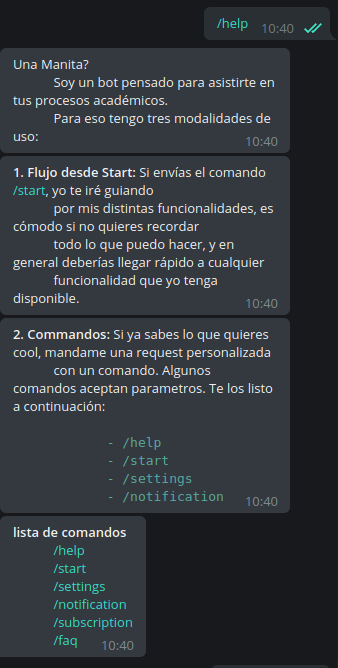
\includegraphics[scale=0.5]{media/imagenes/sc/help.png}
    \caption[Bot help]{Captura de pantalla del Bot Respondiendo el nuevo comando help}
\end{figure}


% \printglossaries[type=\acronymtype]
\printglossaries

\nocite{*}
% \bibliographystyle{babplain}

% \bibliography{bibliografia}
\printbibliography

\newpage
\begin{appendices}
    \chapter*{Anexo}
\end{appendices}

\begin{figure}[h]
    \centering
    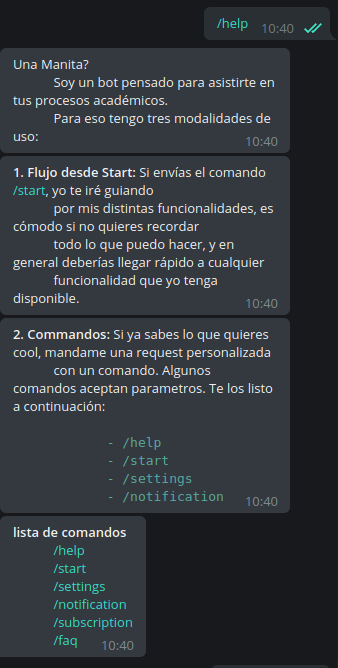
\includegraphics[scale=0.5]{media/imagenes/sc/help.png}
    \caption[Bot help]{Captura de pantalla del Bot Respondiendo el nuevo comando help}
\end{figure}

\end{document}
